\documentclass[10pt,a4paper]{article}

% Packages available in TeX Live
\usepackage[a4paper,margin=18mm]{geometry}
\usepackage{lmodern}
\usepackage{amsmath,amssymb,mathtools}
\usepackage{booktabs,tabularx,array}
\usepackage{graphicx}
\graphicspath{{figures/}}
\usepackage{xcolor}
\usepackage{fancyhdr}
\usepackage{microtype}
\usepackage{caption}
\usepackage[numbers,sort&compress]{natbib}
\usepackage[hyphens]{url}
\usepackage{hyperref}

% Ragright X column for clean wrapping without overfull/underfull hboxes
\newcolumntype{Y}{>{\raggedright\arraybackslash}X}

% Formatting and color palette
\definecolor{primary}{RGB}{22,68,119}
\definecolor{secondary}{RGB}{45,95,145}
\definecolor{rulecolor}{RGB}{180,195,210}

\hypersetup{
    colorlinks=true,
    linkcolor=primary,
    citecolor=primary,
    urlcolor=secondary,
    pdftitle={An input-channel audit of RoseTTAFold3: MSA writing, mutation-effect prediction, and conformational-state selection},
    pdfauthor={Cheng Ding}
}

\setlength{\parskip}{5pt plus 1.5pt minus 1pt}
\setlength{\parindent}{0pt}
\setlength{\tabcolsep}{4.5pt}
\renewcommand{\arraystretch}{1.12}

% Header & Footer
\pagestyle{fancy}
\fancyhf{}
\fancyhead[L]{\footnotesize\textcolor{secondary}{\textit{Input-Channel Audit of RoseTTAFold3}}}
\fancyhead[R]{\footnotesize\textcolor{secondary}{\textit{Ding}}}
\fancyfoot[C]{\footnotesize\thepage}
\renewcommand{\headrulewidth}{0.4pt}

\captionsetup{font=small,labelfont={bf,color=primary},skip=5pt}
\captionsetup[figure]{name=Fig,labelsep=period}

\begin{document}

% Title Block (PLOS Computational Biology standard title page)
\begin{center}
    {\LARGE\textbf{\color{primary}An input-channel audit of RoseTTAFold3: MSA writing, mutation-effect prediction, and conformational-state selection}}\\[10pt]
    {\normalsize \textbf{Cheng Ding}\textsuperscript{1,*}}\\[6pt]
    {\small \textsuperscript{1}School of Life Science and Technology, ShanghaiTech University, Shanghai, China}\\[4pt]
    {\small * Correspondence: \href{mailto:dingcheng2024@shanghaitech.edu.cn}{dingcheng2024@shanghaitech.edu.cn} $\cdot$ ORCID: \href{https://orcid.org/0009-0001-7221-9066}{0009-0001-7221-9066}}
\end{center}

\vspace{4pt}
\noindent\textcolor{rulecolor}{\rule{\textwidth}{0.8pt}}

% Single-paragraph Abstract (<=300 words, no subheadings, no citations)
\section*{Abstract}
AlphaFold3-style structure predictors discard the explicit multiple sequence alignment (MSA) representation after a compact module within each recycle, leaving the pair representation to carry evolutionary information. Here we audit this input channel in RoseTTAFold3 across representation geometry, deep mutational scanning (DMS), and conformational-state selection. Across three proteins, MSA input reduced effective rank by 16--42\% while preserving mutant-conditioned directions and improved cross-position DMS prediction. De-biased gains were $+0.14$--$0.15$ Spearman $\rho$ on RBD and $+0.14$--$0.18$ on CASP3; contiguous-block cross-validation yielded gains of $+0.256$ and $+0.264$, respectively. A single MSA recycle installed approximately 75\% of the geometric and 85\% of the functional effect, with only about 25\% of the geometric effect erased by nine subsequent MSA-free recycles. On RBD, conservation contributed approximately two-thirds and covariation one-third of the alignment-content gain, which approached saturation near eight rows. Distogram analysis of 13 two-state entries and explicit sampling of 480 structures showed that MSA effects on conformational selection were target-dependent and consistent with family consensus. Structural templates constituted a distinct prior: they impaired RBD mutation-effect prediction and strongly steered sampled conformations, but no universal template--MSA hierarchy was observed. Native MSAs preserved or restored the native fold in GA88 and produced a mixed ensemble in GB88 when opposed by an alternative-fold template. Several template-conditioned distogram preferences disagreed with sampled coordinates. These results establish a multi-level account of MSA and template priors in RoseTTAFold3 and show that conformational audits should include explicit coordinate generation.

% Author Summary (150-200 words, non-technical, first-person, no abbreviations)
\section*{Author Summary}
Proteins can adopt different shapes to perform their functions, and computational models are increasingly used to predict these shapes and the effects of mutations. These models can use information from many related protein sequences, but it has been unclear how this information is retained inside newer model architectures. We investigated RoseTTAFold3 and found that evolutionary information leaves a lasting imprint after a single processing step. This imprint improves the prediction of mutation effects and can influence which of several possible protein shapes the model selects. Supplying an example structure, known as a structural template, affects the model in a different way: it can strongly guide the predicted shape but reduce sensitivity to mutations. The outcome of combining evolutionary information and structural templates depends on the protein. We also found that an internal distance-based score can disagree with the three-dimensional structures that the model actually generates. Our findings provide a unified way to examine how different inputs guide structure prediction and highlight the importance of checking generated structures directly.

\noindent\textcolor{rulecolor}{\rule{\textwidth}{0.8pt}}

\section{Introduction}

Deep learning models for biomolecular structure prediction rely on three primary input channels: the target amino acid sequence, homologous multiple sequence alignments (MSAs) \citep{marks2012protein,senior2020improved}, and homologous or experimental structural templates \citep{jumper2021highly,abramson2024accurate}. In the canonical AlphaFold2 (AF2) architecture, the Evoformer maintains a full, explicit MSA representation alongside the residue-pair representation across all 48 blocks, continuously exchanging information between sequence alignments and pairwise geometric features \citep{jumper2021highly}. However, recent architectural generations---including AlphaFold3 (AF3) \citep{abramson2024accurate}, RoseTTAFold3 (RF3) \citep{corley2025atomworks}, and related Pairformer designs \citep{akiyama2025scaling}---reduce the computational footprint of alignment processing. In an AF3-style trunk, the MSA is processed only within a compact four-block module at the beginning of each recycle via outer-product mean and transition operations; thereafter, the explicit MSA representation is discarded, and downstream reasoning within the Pairformer trunk and diffusion structure module relies on the residue-pair representation.

This architectural design raises several mechanistic questions. When a transient MSA input is projected into the pair representation and subsequently discarded, what geometric and biological information is written? Does the pair representation require repeated MSA reinforcement across all recycles, or does the initial recycle establish a persistent state that subsequent MSA-free recycles only partially modify? Furthermore, how does this evolutionary write simultaneously affect two distinct downstream tasks: predicting the functional consequences of single-point mutations---which requires sensitivity to local sequence perturbations \citep{starr2020deep,notin2022tranception,notin2023proteingym}---and selecting among alternative global folds or conformational states in polymorphic proteins \citep{porter2018extant,chakravarty2022alphafold2,wayment2024predicting,chakravarty2024alphafold}?

A parallel set of questions concerns how the MSA channel compares to structural templates and pretrained protein language model (pLM) embeddings \citep{lin2023evolutionary,hayes2025simulating}. In structure prediction and ensemble generation workflows, MSAs and templates are often used as complementary restraints to steer conformational sampling \citep{del2022sampling,stein2022speach,sala2023biasing,heo2022multi,kalakoti2025afsample2}. Yet from an information-theoretic perspective, an alignment of diverged homologs encodes family-wide sequence statistics (encompassing both site-wise conservation and pairwise covariation), whereas a single structural template provides fixed atomic coordinates corresponding to one specific state. Whether a template acts as an equivalent evolutionary prior or as a mutation-suppressing structural constraint within an AF3-style pair representation---and how conflicts between templates and MSAs resolve across different targets---requires systematic evaluation across representation, mutational, and conformational levels.

Here, we perform a multi-level input-channel audit of RoseTTAFold3 (RF3) \citep{corley2025atomworks}. Using a single fixed checkpoint and inference configuration, we trace how input channels modify the trunk pair representation ($\mathbf{Z}_{\mathrm{II}}$) and govern downstream readouts. Across three deep mutational scanning (DMS) benchmarks---SARS-CoV-2 receptor-binding domain (RBD) \citep{starr2020deep,lan2020structure}, human executioner caspase-3 (CASP3) \citep{roychowdhury2022microfluidic}, and bacteriophage $\lambda$ repressor CI \citep{notin2023proteingym}---alongside a 13-entry two-state conformational panel \citep{chang2015protein,burmann2012alpha,luo2004mad2,tuinstra2008interconversion,alexander2007design,saldano2022impact} and 480 sampled 3D structures, our experiments support four main conclusions:
\begin{enumerate}
    \setlength{\itemsep}{2pt}\setlength{\parskip}{0pt}
    \item \textbf{Persistent family-consensus writing:} The MSA leaves a moderate, non-erasing compression in the pair representation that is largely installed in a single recycle ($K=1$) and persists across subsequent MSA-free recycles.
    \item \textbf{Evolutionary content over mere compression:} This write improves cross-position DMS prediction through conservation and covariation content rather than rank compression per se, holding under de-biased standardization and contiguous-block cross-validation.
    \item \textbf{Target-dependent conformational selection:} The same family-consensus prior steers multi-state proteins toward or away from crystallized states depending on family evolutionary context, with major fold-switcher directions verified by explicit 3D coordinate sampling.
    \item \textbf{Distinct template priors and readout decoupling:} Structural templates act as a distinct prior that impairs DMS mutation sensitivity on RBD and exhibits target-dependent conflict resolution against MSAs in 3D coordinate sampling, while showing that distogram log-likelihood readouts can disagree with sampled 3D coordinates in template-conditioned arms.
\end{enumerate}

\section{Results}

\subsection{The MSA leaves a persistent, one-shot family-consensus write in the pair representation}

We first examined how supplying an MSA alters the geometry of single-mutant pair representations ($\mathbf{Z}_{\mathrm{II}}$) and whether this geometric reorganization improves or degrades mutation-effect prediction. Across all three DMS benchmarks, introducing the MSA induced a moderate dimensionality compression without collapsing the representation ensemble (Table~\ref{tab:m1_geometry_dms}; S1~Fig). Specifically, the effective rank (\texttt{eff90}, the number of principal components explaining 90\% of centered mutant ensemble variance) decreased by 26\% in SARS-CoV-2 RBD ($231 \rightarrow 171$), 42\% in homodimeric CASP3 ($333 \rightarrow 193$), and 16\% in $\lambda$ repressor CI ($61 \rightarrow 51$). Linear centered kernel alignment (CKA) \citep{kornblith2019similarity} between the no-MSA and with-MSA ensembles ranged from $0.527$ (RBD) and $0.553$ (CASP3) to $0.917$ (CI), while median directional cosine similarity of individual mutation difference vectors (\texttt{dCos}) ranged from $0.362$ to $0.844$. In full-set RBD, where per-mutant norm ratios were evaluated, the median Euclidean norm of mutant-minus-wild-type perturbation vectors increased rather than shrank ($\Delta$ norm ratio $= 1.21$). Thus, the MSA did not act as a sequence-erasing filter that projected point mutants onto an identical wild-type representation; instead, it re-oriented mutant perturbations within a more compact subspace.

\begin{table}[!ht]
\centering
\caption{Geometric reorganization and cross-position DMS predictive gain induced by MSA input across three benchmark proteins.}
\label{tab:m1_geometry_dms}
\small
\begin{tabularx}{\textwidth}{l c c c c Y l}
\toprule
\textbf{Protein} & \textbf{\texttt{eff90} (no $\rightarrow$ MSA)} & \textbf{Rel. $\Delta$\texttt{eff90}} & \textbf{Linear CKA} & \textbf{\texttt{dCos}} & \textbf{Canonical $\Delta\rho$ (MSA $-$ no)} & \textbf{De-biased $\Delta\rho$} \\
\midrule
SARS-CoV-2 RBD & $231 \rightarrow 171$ & $-26\%$ & 0.527 & 0.474 & $+0.179$; rep. $+0.204$ (5/5 splits) & $+0.14$ to $+0.15$ \\
Human CASP3 & $333 \rightarrow 193$ & $-42\%$ & 0.553 & 0.362 & $+0.162$ (5/5 splits) & $+0.14$ to $+0.18$ \\
$\lambda$ Repressor CI & $61 \rightarrow 51$ & $-16\%$ & 0.917 & 0.844 & $+0.075$ (4/5 splits) & Not fully de-biased \\
\bottomrule
\end{tabularx}
\end{table}

Functionally, this geometric reorganization improved cross-position DMS prediction across all three targets (Table~\ref{tab:m1_geometry_dms}). Under the canonical full-set evaluation, MSA addition increased Spearman $\rho$ by $+0.179$ (and $+0.204$ in an independent full-set replicate, positive in 5/5 splits) on RBD, $+0.162$ (5/5 splits) on CASP3, and $+0.075$ (4/5 splits) on the smaller CI dataset ($N=351$, best-validation protocol).

Because AF3-style trunks re-inject the MSA at the start of each recycle, we performed recycle-gating experiments on the 500-mutant stride-8 RBD subset (Protocol E7; Table~\ref{tab:e1_e7_combined}B; S2~Fig) in which the 15-row MSA was provided for only the first $K \in \{1, 2, 3\}$ recycles, followed by $10 - K$ MSA-free recycles. Exposing the trunk to the MSA for a single recycle ($K=1$) compressed \texttt{eff90} from $181$ to $150$---capturing 74\% (approximately 75\%) of the total geometric compression achieved by 10 full MSA recycles ($\text{\texttt{eff90}} = 139$)---and raised DMS Spearman $\rho$ from $0.414$ to $0.605$, capturing 85\% of the full 10-recycle functional gain ($\rho = 0.638$). Extending exposure to $K=2$ and $K=3$ recycles captured 86--88\% of the geometric shift and 87--96\% of the functional gain (with minor non-monotonic variation between $K=2$ and $K=3$). Nine subsequent MSA-free recycles following $K=1$ washed out only about 25\% of the initial geometric compression. Within the 10-recycle inference regime, MSA writing into the pair representation is therefore predominantly a one-shot event that persists across subsequent recycles.

\begin{table}[!ht]
\centering
\caption{Dissection of MSA dose, biological content (Protocol E1, Panel A), and recycle-gating dynamics (Protocol E7, Panel B) on the RBD 500-mutant stride-8 subset.}
\label{tab:e1_e7_combined}
\small
\begin{tabularx}{\textwidth}{l Y r r r}
\toprule
\textbf{Arm / Exposure} & \textbf{Protocol Description \& Perturbation} & \textbf{\texttt{eff90}} & \textbf{Spearman $\rho$} & \textbf{Gain / Share} \\
\midrule
\multicolumn{5}{l}{\textit{\textbf{Panel A: Protocol E1 Dose $\times$ Content Decomposition} (Gain referenced to \texttt{depth01} zero-content baseline)}} \\
\texttt{noMSA} & Sequence track only (MSA pathway bypassed) & 181 & 0.414 & $-0.076$ \\
\texttt{depth01} & Single query row via MSA pathway (zero-content baseline) & 165 & 0.490 & $0.000$ \\
\texttt{random} & Shared alignment context; synthetic random sequences & 149 & 0.479 & $-0.011$ \\
\texttt{rowshuffle} & Shared alignment context; per-row shuffled residues & 155 & 0.477 & $-0.013$ \\
\texttt{consensus} & Identical copies of the MSA consensus sequence (profile mode) & 156 & 0.501 & $+0.011$ \\
\texttt{colshuffle} & Per-column residue frequencies preserved; covariation destroyed & 150 & 0.596 & $+0.106$ \\
\texttt{depth04} & 4 real homologous sarbecovirus rows & 157 & 0.536 & $+0.046$ \\
\texttt{depth08} & 8 real homologous sarbecovirus rows & 138 & 0.626 & $+0.136$ \\
\texttt{full15} & All 15 real homologous sarbecovirus rows & 139 & 0.638 & $+0.148$ \\
\midrule
\multicolumn{5}{l}{\textit{\textbf{Panel B: Protocol E7 Recycle Gating} (Geometric / functional share of 10-recycle \texttt{full15} effect vs. \texttt{noMSA})}} \\
$K=1$ recycle & 1 MSA recycle followed by 9 MSA-free recycles & 150 & 0.605 & 74\% geom. / 85\% func. \\
$K=2$ recycles & 2 MSA recycles followed by 8 MSA-free recycles & 145 & 0.628 & 86\% geom. / 96\% func. \\
$K=3$ recycles & 3 MSA recycles followed by 7 MSA-free recycles & 144 & 0.609 & 88\% geom. / 87\% func. \\
\bottomrule
\end{tabularx}
\end{table}

\subsection{DMS gains arise from conservation and covariation rather than rank compression or split leakage}

To test whether the observed DMS gains were inflated by validation protocol optimism or sequence-position proximity between training and test sets, we evaluated de-biasing schemes and contiguous-block cross-validation (Protocol E427; S1~Table). First, separating epoch selection from test evaluation and enforcing strict train-only standardization measured two sources of upward bias in canonical best-validation numbers: single-validation best-epoch selection contributed $+0.04$ to $+0.09$ across cells (up to $+0.094$ on the RBD MSA-only probe across 5/5 splits), while full-sample channel standardization shifted RBD MSA-only $\rho$ from $0.589$ to $0.644$ ($+0.055$ across 15/15 paired runs) compared to $+0.022$ for no-MSA. Removing both biases preserved a consistent MSA advantage: on RBD, held-out test evaluation at the validation-selected epoch ($+0.141$), best-test evaluation ($+0.143$), and strict train-only standardization ($+0.146$) yielded de-biased gains of $+0.14$ to $+0.15$. On CASP3, dual-validation de-biased estimates yielded $+0.142$ to $+0.183$. Comparing RBD and CASP3 indicated that validation-set asymmetry is not determined simply by rank compression: CASP3 underwent stronger rank compression than RBD ($-42\%$ vs. $-26\%$) without exhibiting the same standardization shift, and the two proteins showed opposite relationships between stable and noisy single-stream probes.

Second, replacing random position holdout with 5-fold contiguous sequence-block cross-validation (Protocol E427; S1~Table) yielded net MSA gains of $+0.256$ on full-set RBD (5/5 folds: $+0.200$, $+0.328$, $+0.312$, $+0.214$, $+0.226$) and $+0.264$ on CASP3 (5/5 folds: $+0.330$, $+0.141$, $+0.267$, $+0.351$, $+0.231$), exceeding the corresponding random-position holdout gains ($+0.204$ and $+0.162$). Random position holdout therefore did not manufacture the MSA advantage; rather, random splits modestly aided the no-MSA baseline via interpolation from adjacent sequence positions. Evaluating lightweight probes in E427 showed that a per-residue multilayer perceptron (MLP) preserved the MSA gain across all three proteins ($+0.157$ on RBD, $+0.160$ on CASP3, $+0.089$ on CI; all 5/5 splits). A flattened linear probe retained the gain on CASP3 ($+0.163$, 5/5 splits) and directionally on CI ($+0.085$, 3/5 splits), but dropped to $+0.030$ on RBD (3/5 splits, with both arms near $\rho \approx 0.30$), defining a readout boundary where RBD's MSA write requires at least per-residue nonlinear decoding.

To determine whether rank compression itself drove functional gains, we examined the 9-arm dose $\times$ content decomposition on the 500-mutant RBD subset (Protocol E1; Table~\ref{tab:e1_e7_combined}A; S2~Fig). Passing the single wild-type sequence through the MSA featurization pathway (\texttt{depth01}) reduced \texttt{eff90} from $181$ (\texttt{noMSA}) to $165$ and raised $\rho$ from $0.414$ to $0.490$ ($+0.076$), identifying a featurization-path effect and establishing \texttt{depth01} ($\rho = 0.490$) as the zero-biological-content baseline. Relative to \texttt{depth01}, alignment effects separated into three components:
\begin{enumerate}
    \setlength{\itemsep}{2pt}\setlength{\parskip}{0pt}
    \item \textbf{Shared-context compression tax:} Supplying \texttt{random} or \texttt{rowshuffle} alignments compressed \texttt{eff90} to $149$--$155$ without improving DMS prediction ($-0.011$ and $-0.013$ vs. \texttt{depth01}), showing that rank reduction alone does not confer functional gain.
    \item \textbf{Conservation ($\approx 2/3$ of biological gain on RBD):} Preserving per-column amino acid frequencies while destroying inter-column covariation (\texttt{colshuffle}) yielded $\rho = 0.596$ ($+0.106$ over \texttt{depth01}). Because a modal consensus sequence (\texttt{consensus}) gave $+0.011$, the conservation-specific step from \texttt{consensus} to \texttt{colshuffle} contributed $+0.095$, or roughly two-thirds of the $+0.148$ biological gain. Although \texttt{consensus} and \texttt{colshuffle} had similar effective ranks ($156$ vs. $150$), their mutant directional cosines differed substantially ($\text{\texttt{dCos}} = 0.815$ vs. $0.548$), indicating that directional reorganization rather than rank explains their functional difference. Notably, $K=1$ recycle and \texttt{colshuffle} both yielded $\text{\texttt{eff90}} = 150$, providing a geometric triangulation without implying identical information content.
    \item \textbf{Covariation ($\approx 1/3$ of biological gain) and saturation:} Restoring intact homologous rows (\texttt{colshuffle} $\rightarrow$ \texttt{full15}) added $+0.042$ ($\rho = 0.596 \rightarrow 0.638$). Across real row depths, gains rose from $+0.046$ (\texttt{depth04}) to $+0.136$ (\texttt{depth08}) and $+0.148$ (\texttt{full15}), approaching saturation near 8 rows. Across RBD (15 rows, CKA $0.527$), CASP3 (69 rows, CKA $0.553$), and CI (512 rows, CKA $0.917$), DMS gains tracked the magnitude of representation rewriting, consistent with family coherence rather than raw alignment depth being the operative variable in these systems.
\end{enumerate}

\subsection{Family consensus shapes conformational-state selection in fold-switching proteins}

We next investigated how the MSA write affects conformational-state selection across 13 two-state protein entries using range-matched distogram negative log-likelihood (NLL) preferences ($\mathrm{pref} = \mathrm{NLL}_B - \mathrm{NLL}_A$; Fig~1A and S2~Table). Across the 13 entries, 8 targets---including four conformational switches ($\beta_2$AR, Abl1, EGFR, LacY), the 2-row selecase alignment, and three X-ray/NMR static controls (ubiquitin, GB1, thioredoxin)---showed MSA shifts within the empirical repeat-forward noise band ($\pm 0.14$ to $\pm 0.27$). Large MSA shifts occurred in the fold-switching systems:
\begin{itemize}
    \setlength{\itemsep}{2pt}\setlength{\parskip}{0pt}
    \item \textbf{Away from the crystallized state (2 targets):} In KaiB ($\mathrm{pref}: +0.72 \rightarrow -1.57$, $\text{shift} = -2.29$) and RfaH ($+0.10 \rightarrow -2.89$, $\text{shift} = -2.99$), adding the MSA shifted distogram preference away from the crystallized state (State A) toward the solution NMR fold-switched state (State B).
    \item \textbf{Toward the crystallized state (2 targets):} In Mad2 ($-0.05 \rightarrow -0.96$, $\text{shift} = -0.91$, where the crystallized state corresponds to closed State B) and XCL1 ($-0.78 \rightarrow +2.09$, $\text{shift} = +2.87$, toward State A), the MSA shifted preference toward the crystallized state.
    \item \textbf{Own-fold sharpening in a designed pair (1 entry):} In GA88/GB88, the main range-matched flow on GA88 showed sharpening toward its $3\alpha$ fold ($+0.52 \rightarrow +3.07$, $\text{shift} = +2.56$). Under the separate E49b residue-universe scoring flow, GA88 shifted from $+0.38 \rightarrow +2.74$ ($3\alpha$ preference) and GB88 shifted from $-0.23 \rightarrow -2.66$ ($\alpha/\beta$ preference).
\end{itemize}

This bidirectional pattern (2 toward crystal, 2 away, 1 designed-pair sharpening, 8 null) is consistent with the MSA acting as a family-consensus selector rather than a uniform crystal-state bias: in KaiB and RfaH, where the alternative fold-switched form is more prevalent across homologs, the MSA pulls away from the crystallized state, whereas in Mad2 and XCL1 the inferred family consensus aligns with the crystallized state.

To test whether these distogram shifts correspond to actual 3D structures, we sampled 480 structures across 30 condition cells (Protocol E428: 6 target entries $\times$ 5 arms $\times$ 16 structures/cell, 0 failures; Table~\ref{tab:e428_coordinates}; Fig~1B and S3~Table). In the MSA-only arms examined by coordinate sampling, sampled C$\alpha$ structures ($\Delta\mathrm{RMSD} = \mathrm{RMSD}_B - \mathrm{RMSD}_A$) confirmed the primary MSA directions across all four natural fold-switchers: KaiB shifted from 100\% closer to A (\texttt{nomsa} $\Delta\mathrm{RMSD} = +4.174$~\AA{}) to 0\% closer to A (\texttt{msa} $-4.698$~\AA{}); RfaH shifted from 56.2\% closer to A ($+0.185$~\AA{}) to 0\% closer to A ($-9.791$~\AA{}); Mad2 shifted from 87.5\% closer to A ($+0.767$~\AA{}) to 0\% closer to A ($-4.142$~\AA{}); and XCL1 shifted from 0\% closer to A ($-4.000$~\AA{}) to 100\% closer to A ($+6.751$~\AA{}). In the designed pair, coordinate sampling showed that sequence alone (\texttt{nomsa}) placed GB88 in its native B fold (0\% closer to A, $-3.058$~\AA{}) but did not stably select GA88's native A fold (only 6.2\% closer to A, $-2.179$~\AA{}). Supplying each protein's own MSA resulted in 100\% native-state selection for both GA88 ($+6.682$~\AA{}, 100\% A) and GB88 ($-12.387$~\AA{}, 0\% A / 100\% B).

\begin{table}[!ht]
\centering
\caption{Summary of explicit 3D coordinate sampling across six fold-switching systems (Protocol E428: 30 cells $\times$ 16 structures $= 480$ structures) compared against distogram NLL readouts. Positive $\Delta\mathrm{RMSD} = \mathrm{RMSD}_B - \mathrm{RMSD}_A$ indicates 3D coordinates closer to State A (for GA88/GB88, A is the GA88 $3\alpha$ fold and B is the GB88 $\alpha/\beta$ fold). Full per-cell RMSD A and RMSD B values are provided in S3 Table.}
\label{tab:e428_coordinates}
\footnotesize
\begin{tabularx}{\textwidth}{l r r r r r Y}
\toprule
\textbf{System (Metric)} & \textbf{\texttt{nomsa}} & \textbf{\texttt{msa}} & \textbf{\texttt{tplA/Own}} & \textbf{\texttt{tplB/Oth}} & \textbf{\texttt{msa+tpl}} & \textbf{Key Coordinate vs. Distogram Audit Outcome} \\
\midrule
KaiB ($\Delta$RMSD, \AA{}) & $+4.174$ & $-4.698$ & $+6.752$ & $-5.871$ & $+6.349$ & 3D \& distogram concordant; \texttt{msa\_tplA} follows \texttt{tplA} \\
\quad Closer to A (\%) & 100.0\% & 0.0\% & 100.0\% & 0.0\% & 100.0\% & (\texttt{pref}: $+0.72, -1.57, +3.59, -3.00, +3.36$) \\
\midrule
RfaH ($\Delta$RMSD, \AA{}) & $+0.185$ & $-9.791$ & $+12.879$ & $-6.369$ & $+7.598$ & \texttt{tplB} strongly steers 3D coords despite $+0.30$ distogram \\
\quad Closer to A (\%) & 56.2\% & 0.0\% & 100.0\% & 0.0\% & 100.0\% & (\texttt{pref}: $+0.10, -2.89, +1.49, +0.30, +1.45$) \\
\midrule
Mad2 ($\Delta$RMSD, \AA{}) & $+0.767$ & $-4.142$ & $+8.046$ & $-9.643$ & $+7.730$ & Resolves \texttt{tplA} distogram anomaly ($-0.17$): 16/16 at A \\
\quad Closer to A (\%) & 87.5\% & 0.0\% & 100.0\% & 0.0\% & 100.0\% & (\texttt{pref}: $-0.05, -0.96, -0.17, -1.87, -0.17$) \\
\midrule
XCL1 ($\Delta$RMSD, \AA{}) & $-4.000$ & $+6.751$ & $+4.919$ & $-3.453$ & $+4.526$ & \texttt{tplA} steers 16/16 to A (inverting $-1.49$ distogram); \\
\quad Closer to A (\%) & 0.0\% & 100.0\% & 100.0\% & 6.2\% & 93.8\% & \texttt{msa} \& \texttt{tplA} co-directional in 3D despite opposite distograms \\
\midrule
GA88 ($\Delta$RMSD, \AA{}) & $-2.179$ & $+6.682$ & $+6.923$ & $-12.378$ & $+5.593$ & \texttt{msa\_tplOther} preserves native A (16/16), reversing \\
\quad Closer to A (\%) & 6.2\% & 100.0\% & 100.0\% & 0.0\% & 100.0\% & distogram $-4.24$ (\texttt{pref}: $+0.38, +2.74, +4.88, -4.30, -4.24$) \\
\midrule
GB88 ($\Delta$RMSD, \AA{}) & $-3.058$ & $-12.387$ & $-12.761$ & $+8.871$ & $-0.796$ & \texttt{msa\_tplOther} yields 50/50 split, whereas distogram \\
\quad Closer to A (\%) & 0.0\% & 0.0\% & 0.0\% & 100.0\% & 50.0\% & favored A at $+4.58$ (\texttt{pref}: $-0.23, -2.66, -4.34, +4.75, +4.58$) \\
\bottomrule
\end{tabularx}
\end{table}

\begin{figure}[p]
\centering
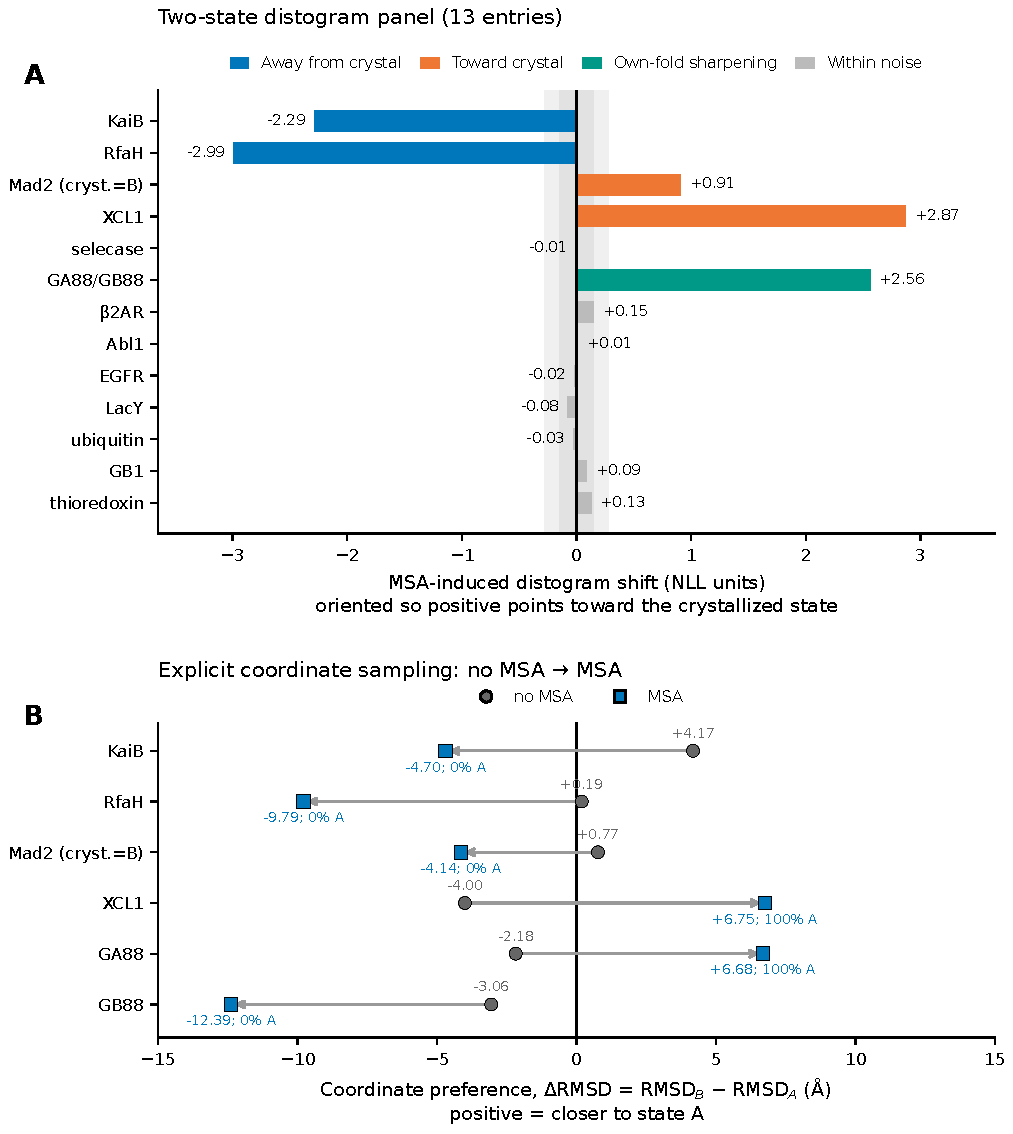
\includegraphics[width=\textwidth,height=0.72\textheight,keepaspectratio]{Fig1_conformational_selection.pdf}
\caption{MSA-driven conformational preference shifts across 13 two-state entries and explicit 3D coordinate verification.
(A) Range-matched distogram preference shifts ($\Delta\mathrm{pref}_{\mathrm{MSA}}$, in NLL units, oriented so positive values point toward the crystallized state; for Mad2, where the crystallized closed state is State B, raw shift is $-0.91$ and crystal-oriented shift is $+0.91$) across the 13-entry two-state panel, categorized into shifts away from crystal (blue: KaiB, RfaH), toward crystal (orange: Mad2, XCL1), own-fold sharpening (teal: GA88/GB88), and shifts within the empirical repeat-forward noise band ($\pm 0.14$ to $\pm 0.27$, shaded gray). (B) Explicit 3D coordinate sampling preferences ($\Delta\mathrm{RMSD} = \mathrm{RMSD}_B - \mathrm{RMSD}_A$ in \AA{}, where positive values indicate structures physically closer to State A; $n=16$ sampled structures per cell, Protocol E428) comparing sequence-only (\texttt{no MSA}, gray circles) to alignment-conditioned (\texttt{MSA}, blue squares) generation across KaiB, RfaH, Mad2, XCL1, GA88, and GB88. Labels report mean $\Delta\mathrm{RMSD}$ and the percentage of sampled structures closer to State A.}
\end{figure}

\subsection{Structural templates are a distinct, target-dependent prior and expose readout decoupling}

We next compared structural templates against MSAs in both conformational selection (Table~\ref{tab:e428_coordinates}; Fig~2A and 2B; S2 and S3~Tables) and RBD mutation-effect prediction (Table~\ref{tab:rbd_msa_vs_template}; Fig~2C and 2D).

In the conformational panel, comparing distogram readouts against 3D sampled coordinates across the template-conditioned arms revealed substantial readout decoupling (Table~\ref{tab:e428_coordinates}; Fig~2A and 2B):
\begin{enumerate}
    \setlength{\itemsep}{2pt}\setlength{\parskip}{0pt}
    \item \textbf{Resolution of apparent natural template anomalies:} On the distogram readout, supplying Template A (\texttt{tplA}) yielded negative preferences in Mad2 ($-0.17$) and XCL1 ($-1.49$), and supplying \texttt{tplB} in RfaH yielded a near-null value ($+0.30$). In explicit 3D coordinate sampling, however, \texttt{tplA} steered 100\% (16/16) of structures to State A in both Mad2 ($\Delta\mathrm{RMSD} = +8.046$~\AA{}, $\mathrm{RMSD}_A = 3.140$~\AA{}) and XCL1 ($\Delta\mathrm{RMSD} = +4.919$~\AA{}, $\mathrm{RMSD}_A = 8.023$~\AA{}), and \texttt{tplB} steered 100\% (16/16) of RfaH structures to State B ($\Delta\mathrm{RMSD} = -6.369$~\AA{}). Thus, the negative Mad2 and XCL1 \texttt{tplA} distogram values were readout artifacts rather than template failures, and in XCL1 the \texttt{msa} and \texttt{tplA} inputs actually favored the same state (State A) in 3D space.
    \item \textbf{Target-dependent conflict resolution between MSA and template:} In the three natural fold-switchers where MSA and \texttt{tplA} opposed each other in 3D coordinates (KaiB, RfaH, and Mad2), the combined \texttt{msa\_tplA} arm followed \texttt{tplA} (100\% closer to State A in all three systems). In the designed pair GA88/GB88, supplying the opposite-fold template alone (\texttt{tplOther}) flipped 100\% (16/16) of sampled structures to the opposite fold ($\Delta\mathrm{RMSD} = -12.378$~\AA{} for GA88; $+8.871$~\AA{} for GB88). When paired with each sequence's own MSA (\texttt{msa\_tplOther}), distogram scores remained near the opposite-fold template ($-4.24$ for GA88; $+4.58$ for GB88), but explicit 3D coordinates showed that GA88 retained its native $3\alpha$ fold in 100\% (16/16) of structures ($\Delta\mathrm{RMSD} = +5.593$~\AA{}, $\mathrm{RMSD}_A = 6.008$~\AA{}) while GB88 shifted to a 50.0\% (8/16) mixed ensemble ($\Delta\mathrm{RMSD} = -0.796$~\AA{}). Consequently, no single cross-target input hierarchy holds across all tested systems.
\end{enumerate}

\begin{table}[!ht]
\centering
\caption{Comparison of MSA and structural template priors on SARS-CoV-2 RBD representation geometry and DMS prediction (500-mutant E49-RBD subset and E427 contiguous block-CV verification).}
\label{tab:rbd_msa_vs_template}
\small
\begin{tabularx}{\textwidth}{l r r r r r Y}
\toprule
\textbf{Input Arm} & \textbf{\texttt{eff90}} & \textbf{CKA vs. no} & \textbf{$\Delta$ Dir.} & \textbf{$\Delta$ Norm} & \textbf{Subset $\rho$} & \textbf{E427 Contiguous Block-CV Verification ($\Delta\rho$)} \\
\midrule
\texttt{no MSA} & 181 & 1.000 & 1.00 & 1.00 & 0.415 & Baseline reference \\
\texttt{MSA (15 rows)} & 139 & 0.568 & 0.48 & 1.21 & 0.638 & $\text{MSA} - \text{no} = +0.259$ (5/5 folds: $+0.121$ to $+0.373$) \\
\texttt{template (6M0J)} & 160 & 0.443 & 0.26 & 1.51 & 0.366 & $\text{tpl} - \text{no} = -0.129$ (4/5 folds: $-0.250$ to $-0.101$, 5th $-0.004$) \\
\texttt{MSA + template} & 159 & 0.448 & 0.26 & 1.52 & 0.370 & $\text{MSA+tpl} - \text{tpl} = +0.003$ (null); $\text{MSA+tpl} - \text{no} = -0.126$ \\
\bottomrule
\end{tabularx}
\end{table}

On the 500-mutant E49-RBD subset, comparing `no MSA`, `MSA 15 rows`, wild-type crystal `template 6M0J` \citep{lan2020structure}, and `MSA + template` showed that templates and MSAs had opposite functional effects on DMS prediction (Table~\ref{tab:rbd_msa_vs_template}; Fig~2C and 2D). Supplying template `6M0J` lowered CKA against no-MSA to $0.443$ ($\text{CKA(template, MSA)} = 0.482$), reduced mutant directional consistency ($\Delta\text{ direction} = 0.26$ vs. $0.48$ for MSA), increased $\Delta$ norm ratio to $1.51$, and reduced DMS Spearman $\rho$ from $0.415$ to $0.366$ ($\Delta\rho = -0.049$ vs. $+0.223$ for MSA). Combining `MSA + template` yielded representation geometry ($\text{\texttt{eff90}} = 159$, $\text{CKA} = 0.448$, $\Delta\text{ direction} = 0.26$, $\Delta\text{ norm} = 1.52$) and DMS correlation ($\rho = 0.370$, $\Delta\rho = -0.045$ vs. no-MSA) close to template alone. Re-evaluating the same four arms under 5-fold contiguous-block cross-validation with the canonical \texttt{SinglePredictorV2} head (Protocol E427; Table~\ref{tab:rbd_msa_vs_template}) yielded $+0.259$ for `MSA - no` (5/5 folds: $+0.121$, $+0.373$, $+0.321$, $+0.223$, $+0.258$), $-0.129$ for `template - no` (4/5 folds: $-0.250$, $-0.152$, $-0.101$, $-0.138$, fifth fold $-0.004$), $+0.003$ for `MSA+template - template` (folds $+0.025$, $-0.042$, $+0.001$, $+0.014$, $+0.016$), and $-0.126$ for `MSA+template - no`. These observations are consistent with a mutation-erasing template prior on RBD that dominates the combined representation and suppresses the DMS gain from the MSA.

\begin{figure}[p]
\centering
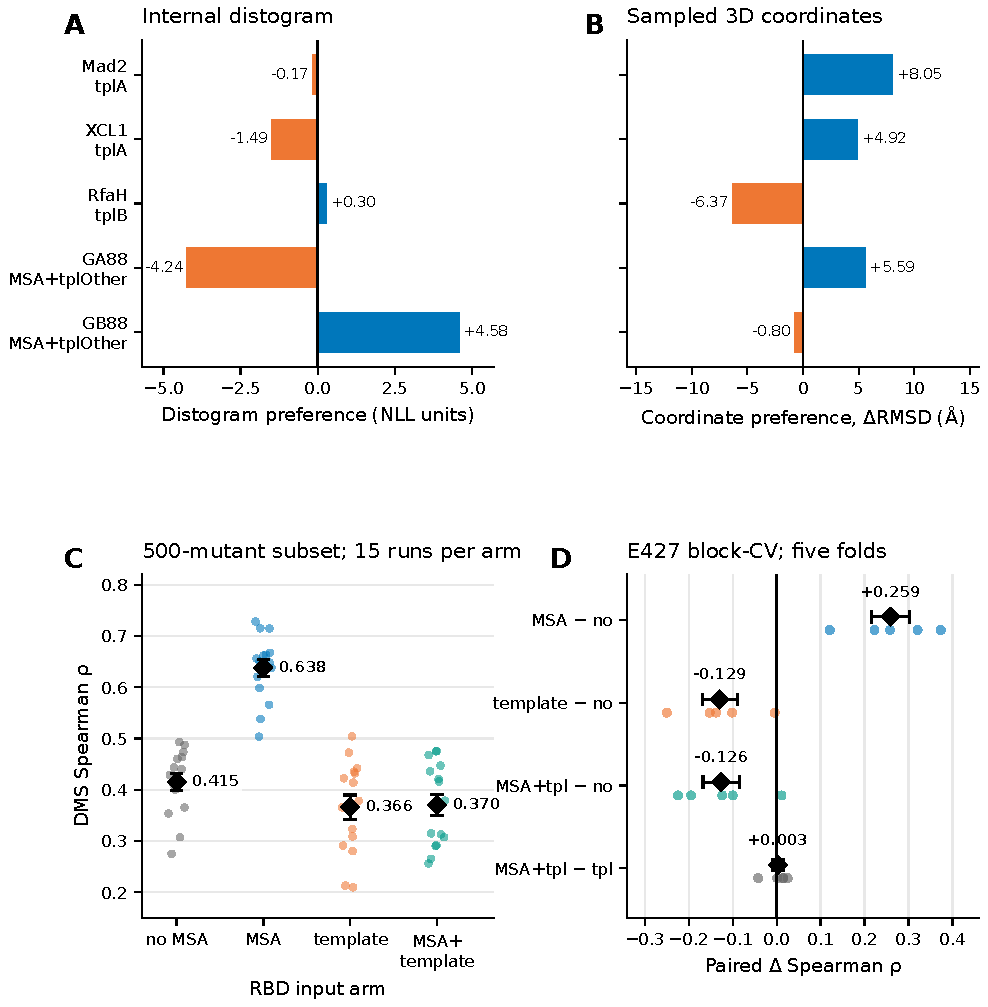
\includegraphics[width=\textwidth,height=0.70\textheight,keepaspectratio]{Fig2_template_conflict.pdf}
\caption{Distogram-coordinate readout decoupling under template conditioning and opposite functional effects of templates vs. MSAs on RBD mutation prediction.
(A) Internal trunk distogram preferences ($\mathrm{pref} = \mathrm{NLL}_B - \mathrm{NLL}_A$, in NLL units) and (B) explicit 3D sampled coordinate preferences ($\Delta\mathrm{RMSD} = \mathrm{RMSD}_B - \mathrm{RMSD}_A$, in \AA{}, Protocol E428; $n=16$ structures per cell) across five diagnostic template-conditioned arms (\texttt{Mad2 tplA}, \texttt{XCL1 tplA}, \texttt{RfaH tplB}, \texttt{GA88 MSA+tplOther}, and \texttt{GB88 MSA+tplOther}), demonstrating directional sign inversions and readout decoupling between trunk distograms and diffusion-sampled 3D coordinates. (C) Cross-position DMS Spearman $\rho$ on the 500-mutant SARS-CoV-2 RBD subset across four input arms (\texttt{no MSA}, \texttt{MSA}, \texttt{template 6M0J}, and \texttt{MSA+template}; 15 runs per arm from 5 splits $\times$ 3 initializations shown as individual points with black diamonds indicating mean $\pm$ SE). (D) Split-paired $\Delta$ Spearman $\rho$ contrasts under 5-fold contiguous sequence-block cross-validation (Protocol E427; individual fold deltas shown alongside mean $\pm$ SE), confirming that the wild-type crystal template impairs RBD mutation-effect prediction ($-0.129$) and suppresses the beneficial MSA write in the combined arm.}
\end{figure}

\subsection{Supporting information accounting and homodimer interface controls}

Four supporting analyses further bounded the information content and behavior of the MSA write (full details in S4 Table and S1 Text):
\begin{itemize}
    \setlength{\itemsep}{2pt}\setlength{\parskip}{0pt}
    \item \textbf{Three-stream marginal accounting ($\mathbf{Z}_{\mathrm{no}}$, $\mathbf{Z}_{\mathrm{msa}}$, \texttt{FAESM}):} In cross-attention fusion with ESM-2 650M embeddings (\texttt{FAESM}) \citep{lin2023evolutionary}, adding $\mathbf{Z}_{\mathrm{no}}$ to $\mathbf{Z}_{\mathrm{msa}} + \text{\texttt{FAESM}}$ produced no detectable additional marginal contribution under the evaluated probe and protocol ($+0.002$ on RBD, $-0.001$ on CASP3, $+0.008$ on CI). Adding \texttt{FAESM} to $\mathbf{Z}_{\mathrm{msa}}$ gave $-0.005$ on RBD (compared to $+0.075$ on $\mathbf{Z}_{\mathrm{no}}$), $+0.051$ (5/5 splits) on CASP3, and an unresolved $-0.039$ on CI driven by a single outlier split (S4 Table).
    \item \textbf{Gradient dominance vs. paired noise floor (Protocol E429):} Late-training encoder gradients favored \texttt{FAESM} over pair streams across all three proteins ($f/z \approx 6.5$, $f/m \approx 2.7$ on RBD; $f/m \approx 3.5$--$3.8$ on CASP3/CI). Scaling the RBD \texttt{FAESM} encoder learning rate by $\lambda = 0.25$ yielded a split-paired gain of $+0.0143 \pm 0.0032$ paired SE ($t = 4.48$, 5/5 splits: $+0.0155$, $+0.0252$, $+0.0091$, $+0.0146$, $+0.0069$), with 75\% Gaussian input noise offering directional support ($0.649 \rightarrow 0.662$, $+0.0128 \pm 0.0110$ SE, 3/5 splits). Protocol E429 (16 identical runs across two processes on RBD \texttt{x\_msa\_faesm}) measured a within-process SD of $0.0016$--$0.0027$ (15/16 runs in $0.6683$--$0.6732$, full range $0.012$ with one outlier at $0.6608$), showing that while $\pm 0.02$ applies to unpaired cell comparisons, the paired learning-rate effect exceeds paired training noise.
    \item \textbf{Partial reconstruction of $\mathbf{Z}_{\mathrm{msa}}$ from $\mathbf{Z}_{\mathrm{no}} + \text{\texttt{FAESM}}$ (Protocol D1):} Across linear, MLP-256/512, and 1--8-layer transformer reconstructors on RBD, validation CKA plateaued near $0.80$--$0.83$ from MLP-512 onward (linear $0.74$; coordinate $R^2$ rising from $0.25$ to $0.36$; 8-layer train--validation CKA gap $+0.09$, suggesting substantial generalization rather than rote memorization; one-hot amino-acid control $\text{CKA} \approx 0.50$). Separate encoders trained with a CKA objective at depths 2/4/6/8 ordered as $\text{both}~(0.811) > \text{\texttt{FAESM}-only}~(0.75\text{--}0.76) > \mathbf{Z}_{\mathrm{no}}\text{-only}~(0.716\text{--}0.717)$. Reconstructed $\hat{\mathbf{Z}}_{\mathrm{msa}}$ achieved $\rho = 0.575$ vs. $0.446$ ($\mathbf{Z}_{\mathrm{no}}$) and $0.663$ (real $\mathbf{Z}_{\mathrm{msa}}$), recovering $59.4\%$ ($\approx 60\%$) of the functional advantage while leaving approximately 40\% of the MSA-specific functional advantage unrecovered at these model scales.
    \item \textbf{CASP3 homodimer interface amplification without paired coevolution:} Across 392 stride-4 CASP3 mutants, the inter-chain $A\text{--}B$ pair block showed higher directional cosine ($0.749$ vs. $0.712$ in $A\text{--}A$/$B\text{--}B$, difference $+0.037$, paired Wilcoxon $p = 5.5 \times 10^{-66}$) and norm amplification ($1.280$ vs. $1.054$/$1.053$). Shuffling chain-B MSA rows across 100 mutants to break species-level pairing preserved identical amplification ($A\text{--}B$: $0.749 / 1.280$; $A\text{--}B - A\text{--}A = +0.037$, $p = 3.9 \times 10^{-18}$; paired vs. unpaired embedding cosine $0.969$), indicating that MSA context amplifies an existing trunk interface prior without requiring paired cross-chain coevolution.
\end{itemize}

\section{Discussion}

\subsection{Persistent MSA writing in an AF3-style pair representation}
Although AF3-style architectures discard the explicit MSA representation after four blocks per recycle, our recycle-gating results on RF3 show that transient MSA processing leaves a persistent imprint in the pair representation. A single recycle ($K=1$) installed roughly 75\% of the geometric compression and 85\% of the DMS predictive gain, and nine subsequent MSA-free recycles erased only about 25\% of the geometric shift. Thus, within the standard 10-recycle regime, the pair representation retains the initial alignment write across subsequent trunk iterations.

\subsection{Evolutionary content rather than rank compression drives mutation-effect gains}
Combining geometric metrics with content perturbations clarifies why compressing the mutant representation ensemble does not erase mutation-effect information. Uninformative alignments (\texttt{random}, \texttt{rowshuffle}) compressed \texttt{eff90} nearly as much as real homologs via the shared-context pathway but produced no DMS gain. Functional improvement required column-level amino acid distributions (\texttt{colshuffle}, contributing $\sim$2/3 of the biological gain on RBD) and inter-column covariation (\texttt{full15}, contributing $\sim$1/3), which reorganized mutant perturbation directions (\texttt{dCos}) rather than merely reducing dimensionality. Similarly, distillation from single-sequence trunk features and ESM-2 embeddings recovered about 60\% of the DMS gain, leaving roughly 40\% of the MSA-specific functional advantage tied to alignment-derived features at the tested capacities.

\subsection{Target-dependent state selection, distinct template priors, and readout boundaries}
Across the conformational panel and explicit 3D sampling ($N=480$ structures), MSA-induced shifts concentrated in fold-switching proteins and aligned in direction with inferred superfamily consensus states (pulling KaiB and RfaH away from crystal states, and Mad2, XCL1, GA88, and GB88 toward their canonical or native folds). While this multi-level consistency supports viewing the MSA as a family-consensus writer and selector, we emphasize that these observations do not constitute a closed causal proof that the exact same latent subspace direction simultaneously causes both DMS gains and conformational switches.

Comparing MSAs with structural templates showed that templates act as a distinct prior rather than an equivalent evolutionary input. On RBD, a wild-type crystal template impaired DMS prediction and overrode the beneficial MSA effect when combined. In conformational selection, templates strongly steered 3D structures, but conflict resolution between templates and MSAs was target-dependent: templates dominated opposing MSAs in KaiB, RfaH, and Mad2, whereas native MSAs preserved the native fold in GA88 (16/16) and produced a 50/50 ensemble in GB88 against an opposite-fold template. Methodologically, the sign inversions between distogram NLL and 3D coordinates in \texttt{tplA} (Mad2, XCL1) and \texttt{msa\_tplOther} (GA88, GB88) demonstrate that distogram readouts are not template-artifact-free; conformational audits of AF3-style models should therefore include explicit 3D coordinate generation, particularly in template-conditioned settings.

\subsection{Limitations}
Several scope boundaries apply to these findings. First, all results come from a single RF3 checkpoint and fixed inference setup and cannot be extrapolated without testing to AF2, AF3, or Boltz \citep{jumper2021highly,abramson2024accurate,kovalevskiy2024alphafold}. Second, DMS analyses used frozen trunk representations across three proteins (RBD, CASP3, CI) with single-point mutants and one assay label each; full de-biasing was completed on RBD and CASP3 but not on the smaller CI dataset ($N=351$), RBD showed a flattened-linear readout boundary in E427, and the $\sim$2/3 conservation vs. $\sim$1/3 covariation split and $\sim$8-row saturation are specific to the 15-row RBD alignment. Third, two-state evaluations simplify multi-state thermodynamic landscapes; explicit 3D coordinate verification (E428) covered 6 of the 13 panel entries at 16 structures per cell, several arms had large absolute RMSDs (so claims are restricted to relative state preference $\Delta\mathrm{RMSD}$ rather than experimental accuracy or Boltzmann populations), and distogram NLL and $\Delta\mathrm{RMSD}$ remain distinct, non-interchangeable readouts. Finally, template behavior may depend on specific PDB chain choices, truncation, and featurization details \citep{watson2023novo}.

\section{Materials and Methods}

\subsection{Model architecture, inference configuration, and feature extraction}
All experiments used a fixed checkpoint of RoseTTAFold3 (RF3) \citep{corley2025atomworks} with 10 recycles, 50 diffusion steps, and a diffusion batch size of 2. Within each recycle, the MSA is processed in four MSA blocks (using outer-product mean operations) to update the residue-pair representation, after which the explicit MSA representation is discarded. We extracted the trunk pair tensor $\mathbf{Z}_{\mathrm{II}} \in \mathbb{R}^{L \times L \times 128}$ immediately after the distogram head projection. For single-point mutants, the true mutated residue index $i$ was sliced along both the row and column axes of $\mathbf{Z}_{\mathrm{II}}$ and stacked into a $2 \times L \times 128$ tensor (for homodimeric CASP3, the $488 \times 488 \times 128$ matrix was archived and sliced at the monomer mutation coordinates; this avoided an early position-0 slicing bug that artificially produced $\text{\texttt{eff90}} \approx 30$). Per-mutant language model representations (\texttt{FAESM}, $L \times 1280$) were extracted from the final layer of ESM-2 650M (\texttt{esm2\_t33\_650M\_UR50D}) \citep{lin2023evolutionary}.

\subsection{DMS datasets and representation geometry metrics}
Three DMS datasets were analyzed: (i) SARS-CoV-2 Spike RBD (201 aa, ACE2 binding \texttt{bind\_avg}, $N=3,998$ single-point mutants, 15 curated sarbecovirus MSA rows, plus a stride-8 subset of $N=500$ mutants for E1, E7, and E49-RBD) \citep{starr2020deep}; (ii) human CASP3 (244 aa/chain homodimer, 488 tokens, fluorescence activity, $N=1,469$ single-point mutants, 69 Swiss-Prot homolog rows) \citep{roychowdhury2022microfluidic}; and (iii) bacteriophage $\lambda$ repressor CI (237 aa construct, 59 assayed positions, ProteinGym \texttt{DMS\_score}, $N=351$ mutants, 512 UniRef30 rows) \citep{notin2023proteingym}.

Over the centered mutant feature matrices, we computed: (i) effective rank (\texttt{eff90}), the number of principal components explaining 90\% of total variance; (ii) linear CKA \citep{kornblith2019similarity} between input conditions; (iii) directional cosine (\texttt{dCos} / $\Delta$ direction), the median cosine similarity of per-mutant difference vectors ($\mathbf{z}_{\mathrm{mutant}} - \mathbf{z}_{\mathrm{WT}}$) across conditions; and (iv) $\Delta$ norm ratio, the median Euclidean norm ratio of $\mathbf{z}_{\mathrm{mutant}} - \mathbf{z}_{\mathrm{WT}}$ relative to the no-MSA baseline.

\subsection{DMS regression, de-biasing, block cross-validation, fusion, and distillation}
Spearman $\rho$ values were compared strictly within each evaluation protocol:
\begin{itemize}
    \setlength{\itemsep}{2pt}\setlength{\parskip}{0pt}
    \item \textbf{Canonical full-set protocol:} Frozen features were trained with the \texttt{SinglePredictorV2} transformer head, per-position/per-channel $z$-score standardization, 70\%/30\% random position holdout (5 splits $\times$ 3 initializations), 300 epochs, AdamW ($\text{lr}=10^{-4}$, $\text{weight\_decay}=0.05$), cosine schedule, MSE loss, and best-epoch validation selection.
    \item \textbf{De-biasing protocols:} Dual-validation separated held-out positions into validation (epoch selection) and test (reporting) subsets; strict train-only standardization computed per-channel mean and variance using training positions only.
    \item \textbf{Protocol E427 (contiguous-block CV and lightweight probes):} Sorted mutated positions were partitioned into 5 contiguous blocks (~20\% positions/fold, 3 initializations). Lightweight readout heads tested a per-residue MLP and a flattened linear probe. E427 also re-evaluated the four RBD template arms using \texttt{SinglePredictorV2} and per-channel standardization.
    \item \textbf{Protocols E1 and E7 (500-mutant RBD subset):} Used a lighter per-position head and per-position scalar standardization; E1 referenced biological gains to \texttt{depth01}.
    \item \textbf{Three-stream fusion, E429 paired noise floor, and D1 distillation:} Multi-stream fusion ($\mathbf{Z}_{\mathrm{no}}$, $\mathbf{Z}_{\mathrm{msa}}$, \texttt{FAESM}) used cross-attention with an orthogonality penalty and dead-stream/zeros controls. Protocol E429 ran 16 identical training replicates across two independent processes (8 runs each) on fixed split and initialization for RBD \texttt{x\_msa\_faesm}. Protocol D1 trained linear, MLP-256/512, and 1--8-layer transformer models (plus one-hot amino-acid controls and CKA-objective separate encoders) to reconstruct $\mathbf{Z}_{\mathrm{msa}}$ from $\mathbf{Z}_{\mathrm{no}}$ and/or \texttt{FAESM}.
\end{itemize}

\subsection{Conformational state selection: distogram preference and 3D coordinate sampling}
The 13-entry two-state panel (S2 Table) was scored on the RF3 64-bin distogram (2--22~\AA{} plus no-contact bin) over the shared resolved residue universe (\texttt{range matching}, avoiding span mismatches and the 14-residue RfaH loop offset) using reference C$\alpha$--C$\alpha$ distance matrices:
\begin{equation}
    \mathrm{pref} = \mathrm{NLL}_B - \mathrm{NLL}_A, \qquad \Delta\mathrm{pref}_{\mathrm{MSA}} = \mathrm{pref}_{\mathrm{MSA}} - \mathrm{pref}_{\mathrm{noMSA}},
\end{equation}
where $\mathrm{pref} > 0$ indicates preference for State A (empirical repeat-forward shift noise band $\pm 0.14$ to $\pm 0.27$). Template inputs required non-zero templated-atom counts and preserved original chain identifiers.

In Protocol E428, explicit 3D coordinates were sampled for KaiB, RfaH, Mad2, and XCL1 across \texttt{\{nomsa, msa, tplA, tplB, msa\_tplA\}} and for GA88 and GB88 across \texttt{\{nomsa, msa, tplOwn, tplOther, msa\_tplOther\}}, with 8 repetitions $\times$ 2 diffusion samples $= 16$ structures per cell ($N=480$ sample-level \texttt{*sample-*\_model.cif} files). Query C$\alpha$ coordinates were aligned to reference CIFs via Needleman--Wunsch alignment and Kabsch superposition over shared residues to compute $\Delta\mathrm{RMSD} = \mathrm{RMSD}_B - \mathrm{RMSD}_A$ ($\Delta\mathrm{RMSD} > 0$ closer to State A).

\section*{Acknowledgments}
The author thanks the developers of RoseTTAFold3, AtomWorks, ESM-2, and ProteinGym for making their model weights, software, and benchmark datasets publicly available. Generative AI tools were used to assist in unifying and editing the manuscript text from the author's experimental archive and fact pack; the author verified all numerical values, citations, and scientific statements and takes full responsibility for the content of the manuscript.

\section*{Funding}
No external funding was received for this work.

\section*{Competing Interests}
The author declares that no competing interests exist.

\section*{Author Contributions}
\textbf{Cheng Ding:} Conceptualization, Data curation, Formal analysis, Investigation, Methodology, Software, Validation, Visualization, Writing -- original draft, Writing -- review \& editing.

\section*{Data Availability Statement}
Analysis code and the numerical outputs underlying all reported summary statistics will be available at \url{https://github.com/Lizon1c/rf3-msa-template-audit}. The 480 sampled coordinate files and analysis-ready feature archives are available at \url{https://doi.org/10.5281/zenodo.23758807}. Publicly available structural and DMS input datasets are identified in Materials and Methods.

\section*{Supporting Information Captions}

\textbf{S1 Fig. Pair-representation effective rank and CKA across three DMS proteins.}
Effective rank (\texttt{eff90}), linear CKA, and directional cosine (\texttt{dCos}) across SARS-CoV-2 RBD, human CASP3, and $\lambda$ repressor CI (archived panel: \texttt{fig1\_geometry\_collapse.png}).

\textbf{S2 Fig. RBD alignment dose-content decomposition and recycle-gating trajectories.}
Effective rank (\texttt{eff90}) and Spearman $\rho$ across the 9-arm Protocol E1 series and Protocol E7 recycle-gating series on the 500-mutant RBD subset (archived panel: \texttt{fig2\_arms\_effrank.png}).

\textbf{S1 Text. Extended methods, analysis artifact notes, and supporting information accounting.}
Detailed description of mutation-site slicing verification, standardization leakage analysis, range-matching alignment fixes, template atom-count checks, Protocol D1 architecture ladder, Protocol E429 paired noise floor, and CASP3 unpaired interface controls.

\textbf{S1 Table. Complete DMS de-biasing and Protocol E427 contiguous-block cross-validation and lightweight probe results.}
Per-split and per-fold Spearman $\rho$ values for canonical, dual-validation, strict train-only standardization, 5-fold contiguous block-CV, per-residue MLP, and flattened linear probes across RBD, CASP3, and CI.

\textbf{S2 Table. Complete 13-entry two-state distogram preference panel and five-target distogram template steering results.}
Range-matched residue counts, MSA depths, $\mathrm{pref}_{\mathrm{noMSA}}$, $\mathrm{pref}_{\mathrm{MSA}}$, shift values, and distogram-level template arms (\texttt{tplA}, \texttt{tplB}, \texttt{msa\_tplA}, \texttt{steer}, \texttt{conflict}).

\textbf{S3 Table. Complete 30-cell explicit 3D coordinate sampling benchmark (Protocol E428, $N=480$ structures).}
Mean $\mathrm{RMSD}_A$, mean $\mathrm{RMSD}_B$, $\Delta\mathrm{RMSD}$, and fraction of structures closer to State A across all 16 structures (8 repetitions $\times$ 2 diffusion samples) for each of the 30 target $\times$ arm cells.

\textbf{S4 Table. Three-stream fusion marginals, Protocol D1 reconstruction ladder, Protocol E429 paired noise-floor replicates, and CASP3 homodimer interface block statistics.}
Complete numerical tables for $\mathbf{Z}_{\mathrm{no}} / \mathbf{Z}_{\mathrm{msa}} / \text{\texttt{FAESM}}$ fusion, RBD learning-rate ($\lambda=0.25$) and input-noise interventions, 16-run E429 paired noise series, D1 CKA/$R^2$/DMS recovery, and paired vs. unpaired CASP3 $A\text{--}A$, $B\text{--}B$, and $A\text{--}B$ blocks.

% References in strict Vancouver citation-sequence order (ordered by first appearance in text)
\begin{thebibliography}{99}

\bibitem{marks2012protein}
Marks DS, Hopf TA, Sander C.
\newblock Protein structure prediction from sequence variation.
\newblock Nat Struct Mol Biol. 2012;19(12):1293--1301.

\bibitem{senior2020improved}
Senior AW, Evans R, Jumper J, Kirkpatrick J, Sifre L, Green T, et~al.
\newblock Improved protein structure prediction using potentials from deep learning.
\newblock Nature. 2020;577(7792):706--710.

\bibitem{jumper2021highly}
Jumper J, Evans R, Pritzel A, Green T, Figurnov M, Ronneberger O, et~al.
\newblock Highly accurate protein structure prediction with AlphaFold.
\newblock Nature. 2021;596(7873):583--589.

\bibitem{abramson2024accurate}
Abramson J, Adler J, Dunger J, Evans R, Green T, Pritzel A, et~al.
\newblock Accurate structure prediction of biomolecular interactions with AlphaFold 3.
\newblock Nature. 2024;630(8016):493--500.

\bibitem{corley2025atomworks}
Corley N, Butterfoss GL, Krishna R, et~al.
\newblock AtomWorks and RosettaFold-3.
\newblock bioRxiv [Preprint]. 2025;2025.08.14.670328.

\bibitem{akiyama2025scaling}
Akiyama Y, Zhang Z, Mirdita M, Steinegger M, Ovchinnikov S.
\newblock Scaling down protein language modeling with MSA Pairformer.
\newblock bioRxiv [Preprint]. 2025;2025.08.02.668173.

\bibitem{starr2020deep}
Starr TN, Greaney AJ, Hilton SK, Ellis D, Crawford KH, Dingens AS, et~al.
\newblock Deep mutational scanning of SARS-CoV-2 receptor binding domain reveals constraints on folding and ACE2 binding.
\newblock Cell. 2020;182(5):1295--1310.e20.

\bibitem{notin2022tranception}
Notin P, Dias M, Frazer J, Marchena-Hurtado J, Gomez AN, Marks D, et~al.
\newblock Tranception: protein fitness prediction with autoregressive transformers and inference-time retrieval.
\newblock In: International Conference on Machine Learning (ICML); 2022. arXiv:2205.13760.

\bibitem{notin2023proteingym}
Notin P, Kollasch AW, Ritter D, van Niekerk L, Paul S, Spinner H, et~al.
\newblock ProteinGym: large-scale benchmarks for protein fitness prediction and design.
\newblock Adv Neural Inf Process Syst (NeurIPS Datasets and Benchmarks). 2023;36.

\bibitem{porter2018extant}
Porter LL, Looger LL.
\newblock Extant fold-switching proteins are widespread.
\newblock Proc Natl Acad Sci U S A. 2018;115(23):5968--5973.

\bibitem{chakravarty2022alphafold2}
Chakravarty D, Porter LL.
\newblock AlphaFold2 fails to predict protein fold switching.
\newblock Protein Sci. 2022;31(6):e4353.

\bibitem{wayment2024predicting}
Wayment-Steele HK, Ojoawo A, Otten R, Apitz JM, Pitsawong W, H{\"o}mberger M, et~al.
\newblock Predicting multiple conformations via sequence clustering and AlphaFold2.
\newblock Nature. 2024;625(7996):832--839.

\bibitem{chakravarty2024alphafold}
Chakravarty D, Schafer JW, Chen EA, Thole JF, Ronish LA, Lee M, et~al.
\newblock AlphaFold predictions of fold-switched conformations are driven by structure memorization.
\newblock Nat Commun. 2024;15:7296.

\bibitem{lin2023evolutionary}
Lin Z, Akin H, Rao R, Hie B, Zhu Z, Lu W, et~al.
\newblock Evolutionary-scale prediction of atomic-level protein structure with a language model.
\newblock Science. 2023;379(6637):1123--1130.

\bibitem{hayes2025simulating}
Hayes T, Rao R, Akin H, Sofroniew NJ, Oktay D, Lin Z, et~al.
\newblock Simulating 500 million years of evolution with a language model.
\newblock Science. 2025;385:eado9336.

\bibitem{del2022sampling}
del Alamo D, Sala D, Mchaourab HS, Meiler J.
\newblock Sampling alternative conformational states of transporters and receptors with AlphaFold2.
\newblock eLife. 2022;11:e75751.

\bibitem{stein2022speach}
Stein RA, Mchaourab HS.
\newblock SPEACH\_AF: Sampling protein ensembles and conformational heterogeneity with AlphaFold2.
\newblock PLOS Comput Biol. 2022;18(8):e1010483.

\bibitem{sala2023biasing}
Sala D, Hildebrand PW, Meiler J.
\newblock Biasing AlphaFold2 to predict GPCRs and kinases with user-defined functional or structural properties.
\newblock Front Mol Biosci. 2023;10:1121962.

\bibitem{heo2022multi}
Heo L, Feig M.
\newblock Multi-state modeling of G-protein coupled receptors at experimental accuracy.
\newblock Proteins. 2022;90(11):1873--1885.

\bibitem{kalakoti2025afsample2}
Kalakoti Y, Wallner B.
\newblock AFsample2 predicts multiple conformations and ensembles with AlphaFold2.
\newblock Commun Biol. 2025;8:373.

\bibitem{lan2020structure}
Lan J, Ge J, Yu J, Shan S, Zhou H, Fan S, et~al.
\newblock Structure of the SARS-CoV-2 spike receptor-binding domain bound to the ACE2 receptor.
\newblock Nature. 2020;581(7807):215--220.

\bibitem{roychowdhury2022microfluidic}
Roychowdhury H, Romero PA.
\newblock Microfluidic deep mutational scanning of the human executioner caspases.
\newblock Cell Death Discov. 2022;8:7.

\bibitem{chang2015protein}
Chang YG, Cohen SE, Phong C, Myers WK, Kim YI, Tseng R, et~al.
\newblock A protein fold switch joins the circadian oscillator to clock output in cyanobacteria.
\newblock Science. 2015;349(6245):324--328.

\bibitem{burmann2012alpha}
Burmann BM, Knauer SH, Sevostyanova A, Schweimer K, Mooney RA, Landick R, et~al.
\newblock An $\alpha$ helix to $\beta$ barrel domain switch transforms the transcription factor RfaH into a translation factor.
\newblock Cell. 2012;150(2):291--303.

\bibitem{luo2004mad2}
Luo X, Tang Z, Xia G, Wassmann K, Matsumoto T, Rieder CL, et~al.
\newblock The Mad2 spindle checkpoint protein has two distinct natively folded states.
\newblock Nat Struct Mol Biol. 2004;11(4):338--345.

\bibitem{tuinstra2008interconversion}
Tuinstra RL, Peterson FC, Kutlesa S, Elgin ES, Kron MA, Volkman BF.
\newblock Interconversion between two unrelated protein folds in the lymphotactin native state.
\newblock Proc Natl Acad Sci U S A. 2008;105(13):5057--5062.

\bibitem{alexander2007design}
Alexander PA, He Y, Chen Y, Orban J, Bryan PN.
\newblock The design and characterization of two proteins with 88\% sequence identity but different structure and function.
\newblock Proc Natl Acad Sci U S A. 2007;104(29):11963--11968.

\bibitem{saldano2022impact}
Salda{\~n}o T, Escobedo N, Marchetti J, Zea DJ, Mac~Donagh J, Velez~Rueda AJ, et~al.
\newblock Impact of protein conformational diversity on AlphaFold predictions.
\newblock Bioinformatics. 2022;38(10):2742--2748.

\bibitem{kornblith2019similarity}
Kornblith S, Norouzi M, Lee H, Hinton G.
\newblock Similarity of neural network representations revisited.
\newblock In: International Conference on Machine Learning (ICML). vol.~97 of PMLR; 2019. p. 3519--3529.

\bibitem{kovalevskiy2024alphafold}
Kovalevskiy O, Mateos-Garcia J, Tunyasuvunakool K.
\newblock AlphaFold two years on: validation and impact.
\newblock Proc Natl Acad Sci U S A. 2024;121:e2315002121.

\bibitem{watson2023novo}
Watson JL, Juergens D, Bennett NR, Trippe BL, Yim J, Eisenach HE, et~al.
\newblock De novo design of protein structure and function with RFdiffusion.
\newblock Nature. 2023;620(7976):1089--1100.

\end{thebibliography}

\newpage
\section*{Supporting Information Tables}

\subsection*{S1 Table. Complete DMS de-biasing and Protocol E427 contiguous-block cross-validation and lightweight probe results}
\begin{table}[!ht]
\centering
\footnotesize
\begin{tabularx}{\textwidth}{l l r l Y}
\toprule
\textbf{Target} & \textbf{Protocol / Probe} & \textbf{$\Delta\rho$ (MSA $-$ no)} & \textbf{Consistency} & \textbf{Fold / Split Breakdown \& Notes} \\
\midrule
RBD & Canonical full-set (\texttt{SinglePredictorV2}) & $+0.179$ / $+0.204$ & 5/5 splits & Two independent full-set runs; best-validation selection \\
RBD & De-biased: test at val-selected epoch & $+0.141$ & 5/5 splits & Removes single-validation epoch-selection optimism ($+0.04$--$0.09$) \\
RBD & De-biased: best held-out test & $+0.143$ & 5/5 splits & Dual-validation split estimate \\
RBD & De-biased: strict train-only z-score & $+0.146$ & 15/15 runs & MSA-only $0.644 \rightarrow 0.589$ ($-0.055$); no-MSA $-0.022$ \\
RBD & E427 Contiguous block-CV (Transformer) & $+0.256$ & 5/5 folds & Folds: $+0.200, +0.328, +0.312, +0.214, +0.226$ \\
RBD & E427 Per-residue nonlinear MLP & $+0.157$ & 5/5 splits & Matches canonical transformer probe magnitude \\
RBD & E427 Flattened linear probe & $+0.030$ & 3/5 splits & Readout boundary: both arms $\rho \approx 0.30$ \\
\midrule
CASP3 & Canonical full-set (\texttt{SinglePredictorV2}) & $+0.162$ & 5/5 splits & Homodimer $488 \times 488 \times 128$ sliced at true mutant positions \\
CASP3 & De-biased: dual-validation range & $+0.142$ to $+0.183$ & 5/5 splits & Across dual-validation estimators \\
CASP3 & E427 Contiguous block-CV (Transformer) & $+0.264$ & 5/5 folds & Folds: $+0.330, +0.141, +0.267, +0.351, +0.231$ \\
CASP3 & E427 Per-residue nonlinear MLP & $+0.160$ & 5/5 splits & Preserves full transformer probe gain \\
CASP3 & E427 Flattened linear probe & $+0.163$ & 5/5 splits & Linearly decodable MSA write \\
\midrule
CI & Canonical full-set (\texttt{SinglePredictorV2}) & $+0.075$ & 4/5 splits & $N=351$ mutants across 59 positions; not fully de-biased \\
CI & E427 Per-residue nonlinear MLP & $+0.089$ & 5/5 splits & Consistent gain across all splits \\
CI & E427 Flattened linear probe & $+0.085$ & 3/5 splits & Direction preserved with lower split consistency \\
\bottomrule
\end{tabularx}
\end{table}

\subsection*{S2 Table. Complete 13-entry two-state distogram preference panel and five-target distogram template steering results}
\begin{table}[!ht]
\centering
\scriptsize
\begin{tabularx}{\textwidth}{l Y r r r r r r r l}
\toprule
\textbf{Target} & \textbf{State A / State B (PDB)} & \textbf{MSA} & \textbf{Res.} & \textbf{no} & \textbf{MSA} & \textbf{Shift} & \textbf{tplA} & \textbf{tplB} & \textbf{MSA+tplA (Steer / Conflict)} \\
\midrule
KaiB & 2QKE XR GS / 5JYT NMR FS & 257 & 90 & $+0.72$ & $-1.57$ & $-2.29$ & $+3.59$ & $-3.00$ & $+3.36$ ($-6.59$ / $-0.23$) \\
RfaH & 2OUG XR $\alpha$ / 2LCL NMR $\beta$ & 257 & 42 & $+0.10$ & $-2.89$ & $-2.99$ & $+1.49$ & $+0.30$ & $+1.45$ ($-1.19$ / $-0.04$) \\
Mad2 & 1DUJ NMR O / 1S2H NMR C & 257 & 184 & $-0.05$ & $-0.96$ & $-0.91$ & $-0.17$ & $-1.87$ & $-0.17$ ($-1.70$ / $0.00$) \\
XCL1 & 1J8I chemokine / 2JP1 $\beta$-sand. & 160 & 39 & $-0.78$ & $+2.09$ & $+2.87$ & $-1.49$ & $-0.86$ & $-1.44$ ($+0.63$ / $+0.05$) \\
LacY & 1PV6 inward / 4OAA outward & 257 & 388 & $+0.06$ & $-0.01$ & $-0.08$ & $+0.54$ & $+0.08$ & $+0.51$ ($-0.47$ / $-0.03$) \\
selecase & 4QHF mon. / 4QHJ olig. & 2 & 105 & $+0.13$ & $+0.13$ & $-0.01$ & --- & --- & Null shift \\
GA88/GB88 & 2JWS $3\alpha$ / 2JWU $\alpha/\beta$ (main) & 24 & 40 & $+0.52$ & $+3.07$ & $+2.56$ & --- & --- & E49b GA: $+0.38\rightarrow+2.74$; GB: $-0.23\rightarrow-2.66$ \\
$\beta_2$AR & 2RH1 inact. / 3SN6 act. & 257 & 271 & $-0.06$ & $+0.09$ & $+0.15$ & --- & --- & Null shift \\
Abl1 & 2GQG DFG-in / 2HYY DFG-out & 257 & 262 & $\approx 0$ & $+0.01$ & $+0.01$ & --- & --- & Null shift \\
EGFR & 1M17 $\alpha$C-in / 1XKK $\alpha$C-out & 257 & 265 & $+0.14$ & $+0.12$ & $-0.02$ & --- & --- & Null shift \\
ubiquitin & 1UBQ XR / 1D3Z NMR & 257 & 76 & $-0.08$ & $-0.10$ & $-0.03$ & --- & --- & Null shift \\
GB1 & 1PGB XR / 2GB1 NMR & 89 & 55 & $+0.36$ & $+0.44$ & $+0.09$ & --- & --- & Null shift \\
thioredoxin & 2TRX XR / 1XOA NMR & 257 & 108 & $+0.26$ & $+0.38$ & $+0.13$ & --- & --- & Null shift \\
\bottomrule
\end{tabularx}
\end{table}

\newpage
\subsection*{S3 Table. Complete 30-cell explicit 3D coordinate sampling benchmark (Protocol E428, $N=480$ structures)}
\begin{table}[!ht]
\centering
\scriptsize
\renewcommand{\arraystretch}{1.04}
\begin{tabularx}{\textwidth}{l l r r r r Y}
\toprule
\textbf{Target} & \textbf{Arm} & \textbf{RMSD A (\AA{})} & \textbf{RMSD B (\AA{})} & \textbf{$\Delta$RMSD (\AA{})} & \textbf{Closer to A} & \textbf{Coordinate Verification Notes ($n=16$ structures/cell)} \\
\midrule
KaiB & \texttt{nomsa} & 4.737 & 8.912 & $+4.174$ & 100.0\% & Sequence-only favors crystallized ground state A \\
KaiB & \texttt{msa} & 9.524 & 4.826 & $-4.698$ & 0.0\% & MSA shifts 16/16 structures to fold-switched state B \\
KaiB & \texttt{tplA} & 2.836 & 9.588 & $+6.752$ & 100.0\% & Template A steers 16/16 to state A \\
KaiB & \texttt{tplB} & 8.944 & 3.073 & $-5.871$ & 0.0\% & Template B steers 16/16 to state B \\
KaiB & \texttt{msa\_tplA} & 3.083 & 9.432 & $+6.349$ & 100.0\% & Joint conflict arm follows \texttt{tplA} \\
\midrule
RfaH & \texttt{nomsa} & 12.296 & 12.482 & $+0.185$ & 56.2\% & Near 50/50 split without MSA \\
RfaH & \texttt{msa} & 15.065 & 5.274 & $-9.791$ & 0.0\% & MSA strongly steers 16/16 to $\beta$-barrel state B \\
RfaH & \texttt{tplA} & 0.824 & 13.702 & $+12.879$ & 100.0\% & Template A closely copies $\alpha$-hairpin state A \\
RfaH & \texttt{tplB} & 13.517 & 7.148 & $-6.369$ & 0.0\% & Template B steers 16/16 to state B (despite $+0.30$ distogram) \\
RfaH & \texttt{msa\_tplA} & 5.786 & 13.383 & $+7.598$ & 100.0\% & Joint conflict arm follows \texttt{tplA} \\
\midrule
Mad2 & \texttt{nomsa} & 12.982 & 13.749 & $+0.767$ & 87.5\% & Modest sequence-only preference for open state A \\
Mad2 & \texttt{msa} & 9.836 & 5.694 & $-4.142$ & 0.0\% & MSA steers 16/16 to closed state B \\
Mad2 & \texttt{tplA} & 3.140 & 11.187 & $+8.046$ & 100.0\% & Steers 16/16 to open state A (resolving $-0.17$ distogram) \\
Mad2 & \texttt{tplB} & 10.656 & 1.013 & $-9.643$ & 0.0\% & Steers 16/16 to closed state B \\
Mad2 & \texttt{msa\_tplA} & 3.581 & 11.311 & $+7.730$ & 100.0\% & Joint conflict arm follows \texttt{tplA} \\
\midrule
XCL1 & \texttt{nomsa} & 13.479 & 9.478 & $-4.000$ & 0.0\% & Sequence-only favors $\beta$-sandwich state B \\
XCL1 & \texttt{msa} & 6.111 & 12.862 & $+6.751$ & 100.0\% & MSA steers 16/16 to chemokine state A \\
XCL1 & \texttt{tplA} & 8.023 & 12.942 & $+4.919$ & 100.0\% & Steers 16/16 to state A (resolving $-1.49$ distogram) \\
XCL1 & \texttt{tplB} & 14.171 & 10.718 & $-3.453$ & 6.2\% & Steers 15/16 to state B \\
XCL1 & \texttt{msa\_tplA} & 9.632 & 14.158 & $+4.526$ & 93.8\% & Co-directional in 3D coordinates (15/16 at state A) \\
\midrule
GA88 & \texttt{nomsa} & 11.400 & 9.221 & $-2.179$ & 6.2\% & Sequence alone does not stably select GA fold (1/16 A) \\
GA88 & \texttt{msa} & 5.255 & 11.937 & $+6.682$ & 100.0\% & Native MSA restores $3\alpha$ fold A (16/16) \\
GA88 & \texttt{tplOwn} & 4.875 & 11.798 & $+6.923$ & 100.0\% & Own template selects $3\alpha$ fold A (16/16) \\
GA88 & \texttt{tplOther} & 13.834 & 1.455 & $-12.378$ & 0.0\% & Opposite template alone flips 16/16 to GB fold B \\
GA88 & \texttt{msa\_tplOther} & 6.008 & 11.601 & $+5.593$ & 100.0\% & Native MSA preserves GA fold A (16/16; distogram $-4.24$) \\
\midrule
GB88 & \texttt{nomsa} & 13.405 & 10.348 & $-3.058$ & 0.0\% & Sequence alone selects native GB fold B (16/16) \\
GB88 & \texttt{msa} & 13.605 & 1.218 & $-12.387$ & 0.0\% & Native MSA sharpens $\alpha/\beta$ fold B (16/16) \\
GB88 & \texttt{tplOwn} & 13.597 & 0.837 & $-12.761$ & 0.0\% & Own template selects $\alpha/\beta$ fold B (16/16) \\
GB88 & \texttt{tplOther} & 3.759 & 12.630 & $+8.871$ & 100.0\% & Opposite template alone flips 16/16 to GA fold A \\
GB88 & \texttt{msa\_tplOther} & 11.586 & 10.790 & $-0.796$ & 50.0\% & Native MSA yields 50/50 mixed ensemble (distogram $+4.58$) \\
\bottomrule
\end{tabularx}
\end{table}

\newpage
\subsection*{S4 Table. Three-stream fusion marginals, D1 distillation, E429 paired noise floor, and CASP3 interface blocks}
\begin{table}[!ht]
\centering
\scriptsize
\begin{tabularx}{\textwidth}{l l Y}
\toprule
\textbf{Audit Module} & \textbf{Condition / Metric} & \textbf{Archived Numerical Result \& Interpretation} \\
\midrule
Three-stream fusion & RBD ($\mathbf{Z}_{\mathrm{no}}, \mathbf{Z}_{\mathrm{msa}}, \text{\texttt{FAESM}}$) & Single-stream $\rho$: $0.465, 0.644, 0.484$; \texttt{FAESM} marginal on $\mathbf{Z}_{\mathrm{msa}}$: $-0.005$ (vs. $+0.075$ on $\mathbf{Z}_{\mathrm{no}}$); $\mathbf{Z}_{\mathrm{no}}$ marginal on $\mathbf{Z}_{\mathrm{msa}}+\text{\texttt{FAESM}}$: $+0.002$. \\
Three-stream fusion & CASP3 ($\mathbf{Z}_{\mathrm{no}}, \mathbf{Z}_{\mathrm{msa}}, \text{\texttt{FAESM}}$) & Single-stream $\rho$: $0.394, 0.556, 0.584$; \texttt{FAESM} marginal on $\mathbf{Z}_{\mathrm{msa}}$: $+0.051$ (5/5 splits); $\mathbf{Z}_{\mathrm{no}}$ marginal on $\mathbf{Z}_{\mathrm{msa}}+\text{\texttt{FAESM}}$: $-0.001$. \\
Three-stream fusion & CI ($\mathbf{Z}_{\mathrm{no}}, \mathbf{Z}_{\mathrm{msa}}, \text{\texttt{FAESM}}$) & Single-stream $\rho$: $0.374, 0.449, 0.452$; \texttt{FAESM} marginal on $\mathbf{Z}_{\mathrm{msa}}$: $-0.039$ (unresolved, driven by one outlier split); $\mathbf{Z}_{\mathrm{no}}$ marginal: $+0.008$. \\
\midrule
Gradient & RBD $\lambda=0.25$ LR scaling & Late-training gradient ratios $f/z \approx 6.5$, $f/m \approx 2.7$ (CASP3/CI $f/m \approx 3.5$--$3.8$). Scaling \texttt{FAESM} encoder LR by $\lambda=0.25$ gives split deltas $+0.0155, +0.0252, +0.0091, +0.0146, +0.0069$; mean $+0.0143 \pm 0.0032$ paired SE ($t=4.48$, 5/5). \\
Gradient & RBD \texttt{FAESM} input noise & 75\% Gaussian noise shifts $\rho$ from $0.649 \rightarrow 0.662$ ($+0.0128 \pm 0.0110$ SE, 3/5 splits); 100\% noise returns to $0.648$ (near dead-stream control $0.655$). \\
Protocol E429 & Paired training noise floor & 16 identical runs (2 processes $\times$ 8 runs) on RBD \texttt{x\_msa\_faesm}: within-process SD $0.0016$ and $0.0027$; 15/16 runs in $0.6683$--$0.6732$ (full range $0.012$ with one outlier at $0.6608$). \\
\midrule
Protocol D1 & RBD $\mathbf{Z}_{\mathrm{msa}}$ distillation & Validation CKA: linear $0.74$, MLP-512 and 1--8-layer transformers $0.80$--$0.83$ (coordinate $R^2: 0.25 \rightarrow 0.36$; 8-layer train--val CKA gap $+0.09$; one-hot AA control CKA $\approx 0.50$). Separate CKA encoders (depths 2/4/6/8): both $0.811 > \text{\texttt{FAESM}-only } 0.75\text{--}0.76 > \mathbf{Z}_{\mathrm{no}}\text{-only } 0.716\text{--}0.717$. Functional DMS $\rho$: $\mathbf{Z}_{\mathrm{no}}~0.446$, reconstructed $0.575$, real $\mathbf{Z}_{\mathrm{msa}}~0.663$ ($59.4\%$ recovery; $\sim$40\% unrecovered). \\
\midrule
CASP3 interface & Paired vs. unpaired MSA & Paired (392 mutants): $A\text{--}A$ cos $0.712$ / norm $1.054$; $B\text{--}B$ $0.712 / 1.053$; $A\text{--}B$ $0.749 / 1.280$ ($A\text{--}B - A\text{--}A = +0.037$, $p=5.5\times 10^{-66}$). Chain-B shuffled unpaired (100 mutants): $A\text{--}A$ $0.713 / 1.055$; $B\text{--}B$ $0.712 / 1.054$; $A\text{--}B$ $0.749 / 1.280$ ($+0.037$, $p=3.9\times 10^{-18}$); paired vs. unpaired embedding cosine $0.969$. \\
\bottomrule
\end{tabularx}
\end{table}

\end{document}
